\cotefile{83}
\scanpage{3}
\[
\alpha^2\deleted{+}+\underbrace{\alpha+1}_{\alpha'}=0
\]

% slanted
\margin{\unsure{Icos-aèdre|Icosaèdre} sur $\mathbb{F}_4$ \uline{gribouillis}}

\[
\begin{aligned}
u^2&=u+\unsure{2|\alpha}\\
u^4&=u^2+\alpha^2=u^{2}+\alpha'=u+\alpha+\alpha'=u+1=u'
\end{aligned}
\]

$u^5=uu'=\alpha\,1$

$u$ d'ordre $15$

\[
\deleted{\unsure{u^3}}\qquad u/u'
\]

\[
u^3=u^2+\alpha u=\underline{u+\alpha}+\alpha u=\alpha'u+\alpha
\]

$u^3$ d'ordre cinq

$u^5$ d'ordre $3$

$\deleted{\unsure{u^3=u'{}^3}}$

$\boxed{\alpha'u+\alpha}$ \deleted{$\unsure{\alpha'u+\alpha}$} opère librement sur $S\smallsetminus\{u,u'\}$ avec $2$ orbites

On veut \qquad $u$

\[
\det(u-v)=0\qquad\text{i.e}\quad \underbrace{\det u}_{1}+\underbrace{\det v}_{1}+\operatorname{Tr}uv=0
\]

\[
\text{-}\qquad\text{i.e.}\quad \operatorname{Tr}uv=0\qquad x\otimes x
\]

\uline{NB}

\[
\begin{aligned}
&\operatorname{Tr}uu'=0\\
&\operatorname{Tr}u.u=\operatorname{Tr}u^2=\operatorname{Tr}(u+\alpha.1)=\operatorname{Tr}u=1\ne0
\end{aligned}
\]

\[
\det(u-v)=\det u\unsure{-|+}\det v+\operatorname{Tr}uv=\operatorname{Tr}uv
\qquad \operatorname{Tr}uv=0
\]

$\deleted{\unsure{\underbrace{u-v}_{1}\quad\underbrace{u-v}_{1}|\det(u-v)}}$

\[
\operatorname{Tr}uv=0\qquad
\operatorname{Tr}(u\underline{v'})=\operatorname{Tr}(u(v+1))=\operatorname{Tr}uv+\operatorname{Tr}u=1+\operatorname{Tr}uv
\]

\figure{
\begin{tikzpicture}\draw[rotate=55] (0,0) ellipse (.55 and .22);\end{tikzpicture}}

$\operatorname{Tr}uv$ et $\operatorname{Tr}uv'$ sont \uline{différents}

donc \quad $\operatorname{Tr}uv=0\Longrightarrow\operatorname{Tr}uv'\ne0$

\margin{$\operatorname{Tr}uu'=0$\\$\operatorname{Tr}u^2=1$}

\mspage{L 22}
% typescript upside down relative to the calculations
Tout ce que je croyais avoir à dire, à un moment ou à un autre\deleted{\unsure{d|t}} de la réflexion, que ce soit sur moi, ou sur tel \deleted{autre}\handwritten{\inserted{de mes collègues, \deleted{\illegible{1}} ou amis}}, ou sur un milieu, ou sur\unsure{,} une époque, je l'ai dit, sans \inserted{jamais} avoir à bousculer mes réticences. \handwritten{\inserted{Pour celles-ci,}} Il a suffi à chaque fois que \deleted{\unsure{je les}}\handwritten{\inserted{je les}} examine avec attention, \deleted{\handwritten{\unsure{elles-mêmes}}} pour qu'elles s'évanouissent\deleted{\unsure{,}} sans plus laisser de traces.

% archive sheet number: 2
\scanpage{4}
\[
\begin{pmatrix}a&b\\c&d\end{pmatrix}\quad
\deleted{\left(\begin{smallmatrix}\unsure{a}&\unsure{c}\\[-2pt]\unsure{b}&\unsure{d}\end{smallmatrix}\right)}\quad
\begin{pmatrix}d&-b\\-c&a\end{pmatrix}\ \frac{1}{ad-bc}
\]

\[
\begin{pmatrix}a&b\\c&d\end{pmatrix}
\begin{pmatrix}a'&b'\\c'&d'\end{pmatrix}
=\quad aa'+bc'\qquad ab'+bd'
\]

$\deleted{\unsure{u'.}}$

\[
\boxed{\begin{aligned}uu'&=u'u=\det u\\u+u'&=\deleted{\unsure{4}}\operatorname{Tr}u.\mathrm{id}\end{aligned}}
\qquad 2\operatorname{Tr}u=2\unsure{\operatorname{Tr}|R}
\]

\deleted{Si $\operatorname{Tr}u=$} Si $\operatorname{Tr}u=0$ alors

\[
u'=-u\Longleftrightarrow\operatorname{Tr}u=0
\]

\[
u^2-\operatorname{Tr}(u)\,u+\det u=0
\]

\[
\begin{aligned}
\operatorname{Tr}u&=1&\det u&=0\\
\det u&\overset{?}{=}& &1
\end{aligned}
\]

$\deleted{\unsure{u}}\quad\deleted{\unsure{\det}}\quad\deleted{u=u'}$

\[
\begin{aligned}
&1+x'\otimes x\\
&\langle x,x'\rangle=1\\
&u\mapsto-u'
\end{aligned}
\]

\[
u^2\unsure{-|+}u=0\qquad \unsure{ux}
\]

$\deleted{u(x)\wedge y=x\wedge\unsure{u'(y)}\quad\unsure{u}}$

\[
\begin{aligned}
&E\longrightarrow\check E\simeq E\otimes\omega^{-1}\\
&E\times E\unsure{-|\longrightarrow}\omega\\
&E\simeq\check E\otimes\omega\\
&E
\end{aligned}
\]

\[
u(x)\wedge y=-u'(y)\wedge x
\]

\[
\underline{15.4=60}
\]

\[
\boxed{\deleted{u(x)\wedge y\unsure{+|-}x\wedge u'(y)=0}}
\]

\[
\boxed{u(\unsure{x})\wedge y=x\wedge u'(y)}\qquad\deleted{\unsure{x}}
\]

\[
\deleted{\unsure{x\otimes y}}\qquad\lambda e+\mu f
\]

\[
\begin{aligned}
&\deleted{x'\otimes x}&&x\wedge x&&D\qquad5\\
&\text{\uline{les projections}}&&\deleted{\unsure{u}}&&4.5=20
\end{aligned}
\]

% archive sheet number: 3
\scanpage{5}
\mspage{L 16}

suis dans \handwritten{\inserted{les pages de}} Récoltes et Semailles. \inserted{Et} \deleted{\unsure{A}}aucun des trois n'est a\unsure{chevé|bhevé} avec le point final\handwritten{,} à la page douze cents et quelques. Les échos, déjà, que \unsure{ma} recueillir mon témoignage (et jusques y compris l'écho par le silence \ldots), \deleted{\unsure{fera}}f\handwritten{eront} partie de la ``suite'' du voyage. \deleted{\unsure{Mais à vrai dire,|Mais, à vrai dire,}}\inserted{Quant à \unsure{un|son} ``terme'',} ce voyage \inserted{sûrement} est de ceux qui ne sont jamais menés à terme - pas même, si ça se trouve, au jour de notre mort.

Et me \deleted{\unsure{re}}voilà \deleted{revenu} enfin \handwritten{\inserted{revenu}} au point de départ: te dire d'avance, si faire se peut, ``de quoi il est question'' dans Récoltes et Semailles. Mais il est vrai aussi, que sans l'avoir cherché, les pages précédentes te l'ont déjà dit peu ou prou. Il sera plus intéressant, peut-être, de continuer \deleted{plutôt} sur ma lancée, \handwritten{\inserted{et}} de \unsure{raconter|raonter}, plutôt que d'annoncer.

Juin 1985\\

\deleted{J'ai commencé à} Les page\unsure{s} qui précèdent de cette lettre (ou ``pré-lettre\unsure{'|''} ont été écrites \deleted{à un moment creux} le mois dernier, \unsure{en|an} un court ``moment creux''. Entretemps, j'ai fini de mettre la dernière main à la quatrième partie de Récoltes et Semailles (``Les Quatre Opérations'') - il ne reste plus que cette lettre à terminer, pour que tout soit prêt enfin pour la frappe et pour la duplication. Depuis \inserted{bientôt} un an et demi que je suis``sur le point de terminer'' ces fameuses notes,\deleted{\unsure{eux|aux} et \unsure{sa|son} introduction,} je n'y croyais plus \ldots

En me mettant, au mois de février l'an dernier, à cette ``introduction'' de nature un peu inhabituelle à un ouvrage mathématique, il y avait (je crois) trois genres de choses surtout sur lesquelles j'avais envie de m'exprimer. D'une part, \deleted{\unsure{comme}} m'expliquer sur mes intentions en revenant à une activité mathématique, et sur l'esprit dans lequel j'avais écrit ce premier volume de ``A la Poursuite des Champs'', et dans lequel je comptais poursuivre un vaste voyage de prospection et de découverte mathématiques, dans les ``Réflexions''.\deleted{(} Il ne s'agirait plus, désormais, de présenter des fondements méticuleux et à quatre épingles de théories en gésine, mais de ``carnets de bord'' plutôt, où \unsure{le|un} travail \deleted{de prospection} se poursuivrait au jour le jour, tel qu'il se fait vraiment, depuis les premières intuitions ou idées de départ, floues souvent \deleted{voire \unsure{à}} et réticentes à se laisser saisir dans les mailles du langage,\deleted{(}alors que c'est le langage adéquat à les saisir qui souvent fait justement défaut et qu'il s'agit de faire se condenser d'un apparent néant de brumes \deleted{parfois} impalpables \ldots{} Depuis ce\deleted{\unsure{s}} stade\deleted{\unsure{s}} donc de ce qui n'est encore que pressenti avant d'être

% archive sheet number: 4
\scanpage{6}
\diagram{$\begin{array}{c|llll}
\operatorname{Tr}u=1 &\det u=0&\Rightarrow u^2-u=0&u\ \text{une projection}&20\\
&\det u=1&u^2-u+1=0&\deleted{u=\mathrm{id}+\text{nilpotent}}&20\\
&&(u+\alpha)(u+&\text{\unsure{val. pr. pour|val. propres}}\ \alpha,\alpha'&\\
&\det u=\alpha&u^2-u+\alpha=0&&\text{\textcircled{12}}\\
&\det u=\alpha'&u^2-u+\alpha'=0&&\text{\textcircled{12}}\\ \cline{5-5}\cline{5-5}
&&&&64
\end{array}$}

\deleted{$\unsure{u,v,v'}$}\quad \uline{NB} \uline{les $u$ sont d'ordre 15}

\[
\begin{aligned}
&u^2\unsure{\ne|+|\deleted{+}}\lambda u+\mu=0\\
&1\qquad u\\
&\unsure{u|\alpha}.1\longmapsto 0\,1+u\\
&u\longmapsto-\mu.1+\lambda u\\
&\begin{pmatrix}0&-\mu\\1&\lambda\end{pmatrix}\\
&1\quad u\quad u'
\end{aligned}
\]

$\deleted{u,u'}\quad\deleted{\unsure{v,v'}}$

\[
\begin{aligned}
\operatorname{Tr}u&=\deleted{\unsure{1}}&\operatorname{Tr}v&=1\\
\det u&=&\det v&=\alpha
\end{aligned}
\]

\[
\begin{aligned}
&\operatorname{Tr}(u+v)\deleted{\unsure{\ne}}=0\\
&\det(u-v)=\underset{1}{\det u}+\underset{1}{\det v}+\operatorname{Tr}uv=\deleted{\unsure{2}}\operatorname{Tr}(uv)
\end{aligned}
\]

\[
\deleted{\det(1+}\quad
\operatorname{Tr}uv=\left\{\begin{matrix}0\\1\\\alpha\\\alpha'\end{matrix}\right.
\quad\left|\begin{aligned}&\lambda u+\mu\\&\lambda u'+\mu\\&\lambda^2\alpha+\mu^2+\lambda\mu\ne0\end{aligned}\right.
\]

\diagram{\fbox{\begin{tikzcd}[ampersand replacement=\&,column sep=small,row sep=small]
\& u\arrow[dl,dash]\arrow[r,dash]\&uv\arrow[dl,dash]\\
1\arrow[r,dash]\&v\&
\end{tikzcd}}}

\diagram{\begin{tikzcd}[ampersand replacement=\&,column sep=small,row sep=small]
{u=u'\ \Rightarrow}\&u\arrow[d,dash]\&u'\arrow[dl,dash]\\
\&1\&
\end{tikzcd}}

\[
\begin{aligned}
\lambda u+\mu\quad &\operatorname{Tr}(\lambda u+\mu)=\deleted{\unsure{\lambda u+\mu}}=\lambda\operatorname{Tr}u=\lambda=1\\
u+\mu\quad &\det(u+\mu)=\underbrace{\det u}_{1}+\mu^2+\mu\underbrace{\operatorname{Tr}u}_{\unsure{1|2}}
=\mu^2+\deleted{\unsure{u}}\mu+\alpha=\deleted{\unsure{0|\alpha}}
\end{aligned}
\]

\[
\begin{aligned}
&u+u'=1\\
&u+1=u'\\
&\operatorname{Tr}(uv)=\\
&u\longmapsto u'=u+1\\
&uv
\end{aligned}
\]

\[
\begin{aligned}
&\deleted{\mu^2+\alpha\mu\unsure{.}}&&\deleted{\alpha^2+\alpha^2}\\
&\deleted{\mu^2+\alpha\mu+\alpha'=0}&&\deleted{\alpha^2=\quad\alpha^2+\alpha\alpha'}\\
&1\quad\mu^2+\mu+\alpha=\alpha&&\alpha'{}^2+\underbrace{\alpha\alpha'}_{1}+1=0\\
&\deleted{\mu^2+\mu\unsure{-}}&&\mu^2+\mu=0
\end{aligned}
\]

$u\longmapsto u'$ antipodisme

\[
\begin{aligned}
uv&=\deleted{u+}\lambda u+\mu\\
u(v-\lambda)&=\mu\\
v-\lambda&=\mu u^{-1}=(\mu\alpha')(u+1)\\
v&=\mu\alpha'u+
\end{aligned}
\]

\[
\begin{aligned}
&\operatorname{Tr}uu'=0\\
&\operatorname{Tr}uv=0\qquad v=u'+\underline w\qquad \operatorname{Tr}w=0\\
&\operatorname{Tr}uw=0
\end{aligned}
\]

\[
\begin{aligned}
u\unsure{'.|.|'}u&=\deleted{\unsure{1}}\alpha.1\\
u^{-1}&=\alpha'u'
\end{aligned}
\]

% archive sheet number: 5
\scanpage{7}
\mspage{L 20}

et plus essentiel. Il était suscité par ces ``interpellations'' par\unsure{f|g}ois déconcertantes, me venant de mon passé \inserted{de mathématicien\deleted{\unsure{s}},} par \deleted{\unsure{la|le} truchement de ceux} voix \deleted{de certains} de ceux qui avaient été mes élèves ou mes amis (ou, du moins, de certains d'entre eux). Au niveau épidermique, ce besoin se traduisait par une envie de \handwritten{``}vider \deleted{un peu} mon sac,\handwritten{''} de dire quelques ``vérités déplaisantes''. Mais plus profondément, sûrement, il y avait le besoin de \mbox{f\,a\,i\,r\,e\quad c\,o\,n\,n\,a\,i\,s\,s\,a\,n\,c\,e} enfin avec un passé, que j'avais choisi jusque là d'éluder. C'est de ce besoin-là, avant tout, qu'est issu Récoltes et Semailles, \deleted{qui}\inserted{lequel} a été ma``réponse'', au jour le jour, à cette pulsion de connaissance en moi,et à l'interpellation sans cesse renouvelée qui me venait du monde extérieur, du``monde \inserted{mathématique''} que j'avais quitté. \deleted{Dès} Mis à part les \handwritten{\inserted{toutes}} premières \deleted{\unsure{deux sept|dix-sept}} pages de \deleted{\unsure{la brève|la partie}} ``Fatuité et Renouvellement'' \inserted{en} formant les deux premiers\deleted{es parties}\inserted{chapitres} (``Travail et découverte'' et ``Le rêve et le Rêveur''), et dès le chapitre qui enchaîne ``Naissance de la crainte'' \deleted{\unsure{par}}\handwritten{\inserted{(p. \unsure{18|10})}}, par lequel commence \deleted{le} un ``témoignage'' qui n'était nullement prévu au programme, c'est ce besoin de faire connaissance de mon passé et de l'assumer pleinement, qui (je crois) a été la force principale en oeuvre dans l'écriture de Récoltes et Semailles.

L'interpellation qui m'était venue du monde des mathématiciens, et qui revenait sur moi avec une force nouvelle tout au cours de l'écriture des parties II,\deleted{\unsure{III,}}\handwritten{\inserted{et}} IV de Récoltes et Semailles, \deleted{prenait} avait pris d'emblée le masque de la suffisance, quand ce n'était celui du dédain (``délicatement dosé''), de la dérision ou du mépris, \handwritten{\inserted{que ce soit}} vis à vis de moi (\deleted{rarement}\handwritten{\inserted{parfois}}) ou \deleted{(à tous les coups ou presque)} \handwritten{\inserted{(surtout)}} vis à vis de ceux qui \deleted{avaient}\inserted{avaient} osé s'inspirer de moi\deleted{\unsure{,}} (sans se douter, \handwritten{\inserted{certes,}} de ce qui les attendait) et qui étaient ``classés'' comme ayant partie liée à moi. Et à nouveau je vois apparaître ici le lien évident et profond, entre le \uline{respect} (ou l'absence \inserted{de respect)}\deleted{\unsure{mépris) de}}\inserted{pour} la personne d'autrui, \deleted{et} celui \deleted{de\unsure{s} des processus créateurs}\inserted{pour l'acte de création} \deleted{primordiaux (dont il vient d'être question) et de leurs fruits, et enfin}\inserted{et pour certains de ses fruits parmi les plus délicats et les plus essentiels, et enfin} le respect pour les règles \deleted{élémentaires d'éthique scientifique}\handwritten{\inserted{les plus évidentes}} de l'éthique scientifique\unsure{,|.} \deleted{Faisant le bilan de ce que m'a \unsure{appris|ap} depuis il y a trois mois, de ce que}\handwritten{\inserted{celles que je serais tenté d'appeler les \uline{``règles de décence''}. Ce sont là autant d'aspects, sûrement, d'un élémentaire et essentiel \uline{respect de soi}.}} Si j'essaie de faire le bilan, en une \deleted{for} seule formule lapidaire, de ce que \unsure{m'a|màa} enseigné\inserted{\unsure{s}} ma réflexion au sujet \deleted{du monde mathéma\unsure{-}} \deleted{\handwritten{\unsure{d'une}}}\deleted{de ce}\handwritten{\inserted{d'un certain}} monde qui fut le mien, auquel je m'étais identifié pendant plus de vingt ans de ma vie, je dirais: c'est un monde qui a \deleted{\uline{perdu le respect}}\mbox{p\,e\,r\,d\,u\quad l\,e\quad r\,e\,s\,p\,e\,c\,t} (\textsuperscript{*}).

% archive sheet number: 6
\scanpage{8}
\[
\begin{aligned}
&\operatorname{Tr}vuvu^{-1}=0\text{ ou }1\\
-&\operatorname{Tr}v\,u(v)=\det(v-u(\unsure{w|v}))\in\{0,1\}
\end{aligned}
\]

\[
\operatorname{Tr}(uv)\in\{0,1\}\qquad\forall u,v\in S
\]

\margin{\uline{NB} $\operatorname{Tr}u^2=1$, $\operatorname{Tr}uu'=0$}

OK si $v=u$ ou $v=u'$\qquad d'autre part,

\[
\begin{aligned}\operatorname{Tr}uv'=\operatorname{Tr}u'v&=\\[-2pt]&\operatorname{Tr}uv+1\\&\ne\operatorname{Tr}uv\end{aligned}
\]

Pour les dix autres, ceux-ci forment un ens. à $10$ éléments sur lequel $k[u]^*/k^*$ opère or $k[u]^*$ est cyclique d'ordre $4^2-1=15$, $k^*$ est ss groupe d'ordre $3$, donc $k[u]^*/k^*$ est cyclique d'ordre $5$. On vérifie que $u^5=\alpha.1$ donc $u$ est d'ordre $15$ ($\alpha$ étant d'ordre $3$) donc $u$ \deleted{est}\inserted{définit} un générateur de $k[u]^*/K^*$.

Ceci dit, pts fixes de \deleted{\unsure{Le commutant}}\inserted{$\operatorname{End}(V)=M$.} \deleted{\unsure{dans}} \inserted{l'un des} de $k[\underline u]^*/k^*$, i.e. \unsure{le|les} commutant de $k[u]$ dans $M$, \unsure{du|de} $u$ est réduit à $k[u]$. On a vu que $k[u]\cap S=\{u,u'\}$ donc $u$ ne fixe aucun pt de $S\smallsetminus\{u,u'\}$, qui se décompose donc en deux orbites d'ordre $5$. Donc $\operatorname{Tr}(uv)$ pour $v\in S\smallsetminus\{u,u'\}$ ne peut prendre que deux valeurs au plus (une par orbite)

\margin{\uline{Cor 1} $M^*/k^*\unsure{=|\simeq|=:}G$ transitif sur $S$\\\uline{Cor. 2.} $G$ simplement transitif}

% archive sheet number: 7
\scanpage{9}
\mspage{PU 79}

sans voix ; \deleted{\unsure{et}} sa raison d'être (semblerait-il) n'est pas d'être \uline{entendu}, mais d' \mbox{ê\,t\,r\,e}. Il est le \mbox{C\,r\,é\,a\,t\,e\,u\,r}, celui qui crée sans témoins, avant qu'aucune créature encore n'entre en dialogue avec lui \handwritten{ou} \deleted{même} se réjouisse avec lui de ses oeuvres.

On dit que la langue des images est la langue de l'enfant\handwritten{,} \deleted{lui décrivant}\handwritten{\inserted{La ``langue'' par laquelle il appréhende}} le monde qui l'entoure. J'ai \deleted{\handwritten{\unsure{bien}}} oublié mon enfance, mais quelque chose pourtant me dit que c'est \deleted{bien} vrai, que c'est \handwritten{\inserted{bien là aussi}} la langue de ma propre enfance. Je ne sais si je la retrouverai un jour. Quelqu'un en moi pourtant la parle, cette langue; comme je la parlais, spontanément et sans effort - avant \deleted{de}\handwritten{\inserted{que je}} l'enterre\deleted{r}, un jour, et l'oublie\deleted{r}. Quelqu'un en moi la parle, mais c'est rare que je prenne le loisir d'écouter.

Je ne suis pas le seul, à l'écouter rarement, voire, jamais. Nous avons si bien appris à ne pas l'écouter, et nous sommes si bien embarqués sur le bateau ``Pensée'' à majuscules, alias ``Abstraction'', à la coque étanche de \mbox{m\,o\,t\,s} finement assemblés et rivés \handwritten{!} \deleted{\unsure{même|alors}} \handwritten{A}lors même que nous voudrions trouver le chemin d'un retour vers la langue oubliée de notre enfance, vers la source des rires et des pleurs, et vers les détresses oubliées, peut-être, que \handwritten{j}amais, jamais des mo\handwritten{t}s ne pourront dire - \deleted{\unsure{que}} ce chemin semble perdu à jamais \ldots

% archive sheet number: 8
\scanpage{10}
sur l'ens des $(u,v\unsure{v|0|{} })\in S\overset{\unsure{2|{}}}{\times}S$ tels que $v\ne u$, $\operatorname{Tr}uv\deleted{\in}=\beta$ donné $\in I$

là \deleted{\unsure{où est inclus dans}} $\unsure{\mathbb P|\mathbb F|\mathrm P}_2(k)$ \deleted{\unsure{tel}} formé des $\operatorname{Tr}uv$ \unsure{pour|:} $u,v\in S$, $v\ne u,u'$

Je dis que $\beta\in$\qquad ens \unsure{des val|des valeurs|dans} $\{0,1\}=\mathbb F_2\subset k$

\[
u\qquad\qquad \frac{1}{\alpha}=
\]

\[
u=\begin{pmatrix}0&1\\\alpha&1\end{pmatrix}\qquad
u'=\begin{pmatrix}1&1\\\alpha&0\end{pmatrix}
\qquad
\begin{pmatrix}a&b\\c&d\end{pmatrix}\begin{pmatrix}a'&b'\\c'&d'\end{pmatrix}
\]

\[
u^{-1}=\alpha'\begin{pmatrix}1&1\\+\alpha&0\end{pmatrix}\deleted{\unsure{\alpha}}
=\begin{pmatrix}\alpha'&\alpha'\\\deleted{\alpha}1&0\end{pmatrix}\qquad\operatorname{Tr}u
\]

$\deleted{e_1\qquad e_2}$

\[
\begin{pmatrix}\lambda&0\\0&1\end{pmatrix}
\begin{pmatrix}0&-1\\\alpha&1\end{pmatrix}
\begin{pmatrix}\lambda^{-1}&0\\0&1\end{pmatrix}
\]

\[
\begin{pmatrix}0&\unsure{-|{}}\lambda\\\lambda^{-1}\alpha&1\end{pmatrix}
\qquad v_0=\begin{pmatrix}0&-\lambda\\\lambda^{-1}\alpha&1\end{pmatrix}
\]
\[
\lambda\ne1\qquad\text{i.e. }\lambda\in\{\alpha,\alpha'\}
\]

\[
\underline{v\quad u}vu^{-1}\qquad\left|\begin{aligned}v&\quad uvu^{-1}\\v'&\quad uv'u^{-1}\end{aligned}\right.
\qquad u'u=\det u=\unsure{\alpha}
\]

\[
\begin{aligned}
vu&=\begin{pmatrix}\unsure{+|-|{}}\lambda\alpha&\unsure{+|-|{}}\lambda\\\alpha&1+\lambda^{-1}\alpha\end{pmatrix}\\
vu^{-1}&=\begin{pmatrix}\deleted{\alpha}\lambda&0\\1+\lambda^{-1}&\lambda^{-1}\end{pmatrix}\\
&\lambda^2\alpha+\lambda^{\unsure{1|{}}}+1+\lambda^{-1}+\lambda^{-2}\alpha\\
&\alpha(\lambda^2+\lambda^{-2})+(\lambda+\lambda^{-1})+1
\end{aligned}
\]

\[
\begin{aligned}
vuvu^{-1}&=vuv(\alpha'u')\\
&(vu)(vu)+vuv\\
&\deleted{u^2=u+}\qquad u\overset{u'}{\underline{(u+1)}}=\alpha\\
&&u^{-1}=\alpha'(u+1\\
&\deleted{\lambda\alpha+}\qquad\lambda+\lambda^{-1}=1\\
&\boxed{\alpha\sigma+\sigma+1}\deleted{\unsure{\lambda+\lambda^{-1}}}\qquad\alpha.
\end{aligned}
\]

% archive sheet number: 9
\scanpage{11}
\mspage{7\deleted{\unsure{6|5}}\handwritten{7}}

\deleted{est seul à connaître et à manier, une langue qui d'instant en instant se forme et se transforme sous ses mains de magicien. Invisible, insaisissable, en\handwritten{f}ant espiègle \handwritten{et} \deleted{sage débonnaire} vieux sage énigmatique \deleted{\unsure{et}} \deleted{débonnaire} - c'est \uline{lui}, le Maître du verbe vivant, de la langue sans paroles, \deleted{où \unsure{dans}}\inserted{la \mbox{l\,a\,n\,g\,u\,e\,.\ -\ m\,è\,r\,e} où} les mots innombrables des innombrables langues-mots viennent \inserted{depuis la nuit des âges} puiser \deleted{leur sens,} leur \deleted{\unsure{force}}\handwritten{\inserted{vigueur}} et leur \handwritten{sens}.}

\margin{\handwritten{\unsure{espacer|espaces}}}

C'est une chose étrange que la langue-mère, la langue commune à tous les êtres humains (voire\handwritten{\inserted{même}}, à tous les êtres \ldots), \handwritten{\inserted{qu'elle}} soit à tel point inapte, pourrait-il sembler, comme mode de \uline{communication} \uline{d'un} \uline{sens}, d'\deleted{\unsure{u}}un être à un autre. Ce n'est pas, il est vrai, la langue du patron, et si elle est moyen de communication, ce n'est sûrement pas d'un patron à un autre.

Nous pouvons, bien sûr, la ``traduire'' dans le langage des mots, \deleted{\unsure{et}} \handwritten{C}'est bien ce que je ne manque pas de faire avec \deleted{le}\handwritten{un} \deleted{plus grand} soin\handwritten{\inserted{infini}}, chaque fois (ou presque \ldots) qu'un rêve \deleted{semble} m'interpelle\deleted{\unsure{r}} avec une force exceptionnelle. Une telle ``traduction'' est un moyen d'écoute, tel un stét\handwritten{\inserted{h}}oscope pour des oreilles un tantinet sourdes ! \deleted{Visiblement,} C'est bien utile et même indispensable, vu le cas\handwritten{.} \handwritten{M}ais il est \deleted{\unsure{s}}sûr aussi que la langue-images n'\deleted{\unsure{x}}est pas \deleted{plus} faite pour être traduite en mots, \handwritten{\inserted{pas plus}} que la langue-\deleted{\unsure{paroles}}\handwritten{mots} n'est faite pour le stét\handwritten{\inserted{h}}oscope. \deleted{\unsure{La}}\handwritten{\inserted{Et Toute}} traduction est aussi différente de la parabole originelle, qu'une description d'un feu, d'une eau ou d'une scène vécue, sont différents de la chose décrite.

Si j'essaye d'évoquer quelque moyen de communication directe par la langue-images, ou par quelque \handwritten{\inserted{autre}} ``langue'' qui s'en rapproche tant soit peu, je ne vois guère (faute d'imagination sans doute) que la peinture ou la sculpture, et surtout la \mbox{d\,a\,n\,s\,e} - la langue-mouvement par excellence, la langue du \mbox{c\,o\,r\,p\,s}.

Il est vrai que le corps a mille autres\deleted{\unsure{f}} façons encore de s'exprimer, de ``parler'' - \handwritten{par} un langage plus éloquent parfois que le langage des mots ou même la danse. Il y a le jeu d'amour, certes, ce Jeu des jeux, le jeu \deleted{de}\handwritten{\inserted{que joue}} la Terre \deleted{\unsure{avec|et} de}\handwritten{\inserted{avec}} ses amants innombrables, \handwritten{\inserted{avec}} le soleil, \handwritten{avec} le ciel \deleted{et}\handwritten{\inserted{avec}} la pluie, et \handwritten{\inserted{avec}} \deleted{toutes}\handwritten{\inserted{chacune de}} ses créatures \ldots{} Et il y a la langue des yeux\handwritten{\inserted{aussi}}, comme il y a celle des mains (sans compter celle des pieds\deleted{sous la table}, me souffle un petit diable blagueur \ldots),

\handwritten{D}écidément la liste \handwritten{\inserted{déjà}} s'étoffe! Et je pensais aussi, et surtout, au langage (que la Science baptise de ``psychosomatique'') par lequel le corps exprime et par là, peut-être, ``compense'' \deleted{en quelque sorte}\handwritten{\inserted{à sa façon}}, la violence subie par lui, ou par les couches profondes de la psyché qui s'enracinent en lui, aux mains de forces inquiètes et impitoyables, battant \handwritten{\inserted{souvent}} pavillon ``Esprit''. Et peut-être est-il vrai qu'il n'y a de ``sens'' bel et bien exprimé, \handwritten{\inserted{par qui que ce soit et}} dans quelque langue que ce soit, qui ne soit aussi bel et bien ``entendu'' \ldots

% archive sheet number: 10
\scanpage{12}
\[
\begin{aligned}
v&=\lambda u+\mu&\operatorname{Tr}v&=1\qquad\text{i.e. }\lambda=1\\
v&=u+\mu&\det(\unsure{w|v})&=\underbrace{\det u}+\underbrace{\det\mu.1}_{\mu^2\det1}+\underbrace{\operatorname{Tr}\mu u}_{\mu\underbrace{\operatorname{Tr}u}_{1}}\\
&&&=\alpha+\mu^2+\mu
\end{aligned}
\]

La condition $\underline{\det(v)=\alpha}$ équivaut à

\[
\mu^2+\mu=0\qquad\mu\in\{\underline{0,1}\}\qquad\text{i.e.}\qquad v\in\{u,u'\}
\]

La condition $\det(v)=\alpha'$ équivaut \unsure{à}

\[
\mu^2+\mu+1=0\qquad\text{i.e.}\qquad\mu\in\{\alpha,\alpha'\}
\]

\[
v=u+\alpha,\quad \underbrace{u+\alpha'}_{u'+\alpha}\in S'
\]

\[
\operatorname{Tr}uv=0\qquad\begin{matrix}0&1&\alpha&\alpha'\\&&\alpha^2=\unsure{1|\alpha'}&\end{matrix}
\]

\[
\operatorname{Tr}\underbrace{(u+\alpha)(v+\alpha)}_{uv+\alpha u+\alpha v+\alpha^2}
=\operatorname{Tr}uv+\deleted{\unsure{\alpha}}=\deleted{\unsure{\operatorname{Tr}uv+\alpha}}
\]

\[
\operatorname{Tr}(u+\alpha,v)=\operatorname{Tr}uv+\alpha
\]

\[
\begin{aligned}
&&v&\quad uvu^{-1}\\
\deleted{\operatorname{Tr}v(uvu^{-1})=\operatorname{Tr}((vu)^2u^{-2}}&&v'&\quad u(v)'=u(v')
\end{aligned}
\]

\figure{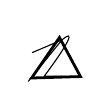
\begin{tikzpicture}[scale=.62]\draw[line width=1pt] (0,0)--(1,.03)--(.57,.83)--cycle;\draw (-.07,-.07)--(.62,.78) .. controls (.91,1.02) and (.76,.71) .. (.26,.04)--(1,.03);\draw (.01,.52)--(.62,.78);\end{tikzpicture}}

\diagram{$\begin{array}{c|cccc}\lambda&0&1&\alpha&\alpha'\\\hline \sigma&&&&\end{array}$}

\figure{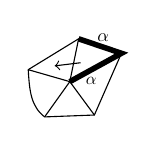
\begin{tikzpicture}[scale=.8]
\coordinate (a) at (0,.72);\coordinate (b) at (.8,1.21);\coordinate (c) at (1.48,.98);\coordinate (d) at (1.05,0);\coordinate (e) at (.26,-.03);\coordinate (o) at (.66,.53);
\draw (a)--(b)--(c)--(d)--(e).. controls (.04,.14) and (.02,.39)..cycle;
\draw (a)--(o)--(b) (o)--(d) (o)--(e);
\draw[line width=2pt] (b)--(c)--(o);
\draw[->] (.83,.83)--(.42,.78);
\node[scale=.65] at (1.19,1.23){$\unsure{\alpha}$};\node[scale=.6] at (1,.54){$\unsure{\alpha}$};
\end{tikzpicture}}

\[
\boxed{\operatorname{Tr}v_0\,u(v_0)=\alpha}\Longrightarrow
\operatorname{Tr}v_{\unsure{i|1|{}}}\,u(v)=\alpha
\quad\text{pour les cinq conjugués de }v
\]

\[
\underset{\operatorname{Tr}(uv)}{\det(u+v)}=
\begin{cases}
\deleted{\unsure{\beta|0}}\alpha&\text{si }\{u,v\}\ \text{\unsure{arête|arêtes}}\\
\alpha'&\text{si }\{u,v\}\ \text{\unsure{coarête|coarêtes|coarêts}}\\
1&\text{si }u=v\\
0&\text{si }u=u'
\end{cases}
\]

\[
\operatorname{Tr}v'\underbrace{u(v')}_{u(v)'}=\alpha
\]

% archive sheet number: 11
\scanpage{13}
% typescript upside down in the scan; order follows the typescript
\mspage{PU 78}

Peut-être que \deleted{\unsure{je}} je \handwritten{\inserted{suis en train là}} digresser - car qui me dit que toutes ces ``langue\handwritten{s}'' que je viens d'évoquer à l'instant, font bien partie de cette ``langue-paraboles'', la langue-mère, qui les engloberait toutes\handwritten{?} Je soupçonne pourtant qu'il en est bien ainsi \ldots{} Mais je reviens à\deleted{\unsure{x}} la forme familière, la \handwritten{``}\uline{parabole}\handwritten{''} - \deleted{\unsure{celle}} où la présence d'un \mbox{s\,e\,n\,s}, exprimé par un génial Metteur-en-scène-Prestidigitateur, saute aux yeux (alors même qu'on s'efforcerait à tout prix de l'ignorer). Si pendant longtemps j'ai été réticent \deleted{\unsure{d'}}\handwritten{à} y reconnaître une véritable \mbox{l\,a\,n\,g\,u\,e} (et je sens que cette réticence, maintenant encore, n'est pas entièrement résorbée \ldots), c'est sans doute, justement, parce qu'elle semble si peu apte à ce qui paraît la raison d'être même de toute langue et de tout langage: la communication avec autrui.

Et pourtant, je sais bien qu'il est plus important encore de savoir ``communiquer'' avec \uline{soi-même}.

Quand l'initiative pour ``parler avec moi-même'' vient de ``moi'', à l'état de veille, l'idée\deleted{\unsure{x}} ne me \deleted{serait venue}\handwritten{\inserted{viendrait}} \deleted{de faire appel} (jusqu'à tout récemment encore, du moins) de faire appel à autre chose qu'à la langue-mots, celle donc que ``je'' connais et manie à l'aise (que ce soit en allemand, ou en français). Mais je sais bien aussi que quand l'initiative vient non de moi, mais de ``l'Autre'', ce n'est jamais \deleted{cette} dans cette langue-là qu'\deleted{\unsure{i}}\handwritten{I}l me parle. C'est toujours dans la langue-paraboles, la ``langue des images'' - et quand je prends la peine d'écouter, souvent je sue\handwritten{\inserted{\unsure{r|*}}} sang et eau pour la ``traduire'' dans \deleted{l'autre}\handwritten{\inserted{``la mienne''}} tant bien que mal. Je ne sais si un jour ce ne sera plus la peine \ldots

\deleted{Peut-être est-ce là,\deleted{\unsure{pa}} pour la langue-paraboles, \deleted{mais \unsure{nulle}} (en tant que ``langue'' tout au moins, \deleted{c'est à dire} comme moyen d'une \uline{communication}) sa seule et grande fonction: de} \handwritten{\inserted{Il semblerait que la ``raison d'être'' de la langue-paraboles soit d'être le moyen entre tous pour}} \mbox{n\,o\,u\,s}\quad\mbox{p\,a\,r\,l\,e\,r} à \mbox{n\,o\,u\,s-m\,ê\,m\,e}\quad\mbox{e\,t}\quad\mbox{s\,u\,r}\quad\mbox{n\,o\,u\,s-m\,ê\,m\,e}. C'est la langue \deleted{\unsure{entre toutes}} que choisit notre ``inconscient'', pour ``parler au conscient''\unsure{.|,} \handwritten{L}a langue \handwritten{\inserted{par laquelle \deleted{se font connaître} s'expriment et se font connaître}} les couches créatrices profondes - celles qui ``\uline{savent}'' et qui ``\uline{peuvent}''\handwritten{,}\deleted{\unsure{;}} domicile et demeure de l'\mbox{A\,u\,t\,r\,e}\deleted{\unsure{(}} \handwritten{,} du \mbox{J\,o\,u\,e\,u\,r}, du \mbox{R\,ê\,v\,e\,u\,r}, du \deleted{\unsure{M}} \uline{Metteur-en-scène} ou \uline{Prestidigitateur} ou quelque autre nom qu'on lui donne; l'\mbox{O\,e\,i\,l} qui voit et l'\mbox{O\,r\,e\,i\,l\,l\,e} qui entend et la \mbox{M\,a\,i\,n} qui tient les clefs de tous les \inserted{coffres et tous les} souterrains, et la torche \handwritten{\inserted{aussi}} pour \deleted{\unsure{en}} voir le fond de tous et de chacun \ldots

C'est même étrange que l'Autre jamais ne se lasse de ``nous'' parler, alors que jamais nous ne l'écoutons, autant dire. Souvent pourtant je sens \deleted{qu'Il \unsure{s}} à quel point Il se régale à ses propres jeux - non \deleted{sans doute}\inserted{certes} à les contempler, mais à les inventer et à les monter \inserted{de toutes pièces} avec \handwritten{cette} verve \deleted{\handwritten{\unsure{inventive}}} qui n'est qu'à lui, et sans nul souci, faut\handwritten{-}il croire, s'il y aura un spectateur-auditeur. Il est la \mbox{\handwritten{V}\deleted{\unsure{v}}\,o\,i\,x} de ce qui \uline{est} en nous et qui semble

% archive sheet number: 12
\scanpage{14}
\figure{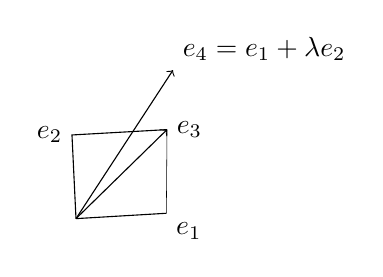
\begin{tikzpicture}[scale=.85]
\draw (0,0)--(1.35,.08) node[below right]{$e_1$};
\draw (0,0)--(-.06,1.25) node[left]{$e_2$}--(1.36,1.33) node[right]{$e_3$};
\draw[very thin] (1.35,.08)--(1.36,1.33);
\draw[->] (0,0)--(1.36,1.33);\draw[->] (0,0)--(1.45,2.22) node[above right]{$e_4=e_1+\lambda e_2$};
\end{tikzpicture}}

\[
\begin{aligned}e_3&=\begin{pmatrix}1\\1\end{pmatrix}\\e_4&=\begin{pmatrix}1\\\lambda\end{pmatrix}\end{aligned}
\]

\[
\boxed{\deleted{\unsure{\xi}}u=\begin{pmatrix}\unsure{\zeta|\xi}&0\\0&-\zeta\end{pmatrix}}
\qquad\begin{aligned}\operatorname{Tr}u&=0&\det u&=-\zeta^2\\\operatorname{Tr}v&=0&\det v&=-\eta^2\end{aligned}
\]

\[
\begin{aligned}
&\deleted{v=\bigl(\unsure{\eta}}\\
&v=\begin{pmatrix}a&b\\c&d\end{pmatrix}\deleted{\bigl(\unsure{0}}\qquad\deleted{v(e_1)=ae_1+ce_2}\\[-2pt]
&&\deleted{v(\unsure{.}}
\end{aligned}
\]

\[
\begin{aligned}
v(e_3)&=(a+b,c+d)=(\eta,\eta)\\
v(e_4)&=(a+\lambda b,c+\lambda d)=(-\eta,-\lambda\eta)
\end{aligned}
\qquad
\begin{aligned}a+b&=\eta\\c+d&=\eta\\a+\lambda b&=-\eta\\c+\lambda d&=-\lambda\eta\end{aligned}
\]

\[
\deleted{v=\begin{pmatrix}a&c\\c&a\end{pmatrix}}\qquad
\begin{aligned}b&=\eta-a\\d&=\eta-c\end{aligned}
\]

\[
\boxed{v=\begin{pmatrix}a&b\\-\lambda b&-a\end{pmatrix}}
\quad\left\{\begin{aligned}a&=\frac{\lambda+1}{\lambda-1}\eta\\
b&=\frac{-2}{\lambda-1}\eta\end{aligned}\right.
\]

\[
\begin{aligned}
a+\lambda(\eta-a)&=-\eta &(1-\lambda)\unsure{(|{}}a&=-(1+\lambda)\eta\\
c+\lambda(\eta-c)&=-\lambda\eta &(1-\lambda)c&=-2\lambda\eta
\end{aligned}
\]

\[
\begin{aligned}
\det v&=-a^2+\lambda \deleted{\unsure{4}}b^2=-\eta^2
\left[\underbrace{\left(\frac{\lambda+1}{\lambda-1}\right)^2-\lambda\frac{4}{(\lambda-1)^2}}_{\displaystyle\frac{(\lambda+1)^2-4\lambda}{(\lambda-1)^2}=1}\right]\\
&=
\end{aligned}
\]

\[
\begin{aligned}
a&=\frac{\lambda+1}{\lambda-1}\eta &b&=\unsure{.}\\
c&=\frac{+2\lambda\eta}{\lambda-1}\\
b&=\eta\left(1-\frac{\lambda+1}{\lambda-1}\right)=\frac{-2\deleted{\unsure{\lambda}}\eta}{\lambda-1}\deleted{\unsure{\eta}}\\
d&=\eta\left(1-\frac{\deleted{\unsure{4}}2\lambda}{\lambda-1}\right)=-\frac{\lambda+1}{\lambda-1}\eta=\deleted{\unsure{a}}\unsure{-|{}}a
\end{aligned}
\]

\[
\begin{aligned}
&\deleted{uv+vu}\\
uv&=\begin{pmatrix}\zeta a&\zeta b\\\deleted{\unsure{a}}\lambda\zeta b&\zeta a\end{pmatrix}
\qquad c=-\lambda b\\
vu&=\begin{pmatrix}\zeta a&-\zeta b\\-\lambda\zeta b&\zeta a\end{pmatrix}
\end{aligned}
\]

\[
uv+vu=\begin{pmatrix}2\zeta a&0\\0&2\zeta a\end{pmatrix}
=\deleted{\unsure{2\zeta\eta\frac{\lambda+1}{\lambda-1}.1|2\zeta a\frac{\lambda+1}{\lambda-1}.1}}\;2\zeta a.1
\qquad 2\zeta a=\operatorname{Tr}vu
\]

% archive sheet number: 13
\scanpage{15}
\mspage{PU 74}

Par sa ``texture sensorielle'', l'image\deleted{\unsure{ sym}} peut consister en des sons, \handwritten{ou} des odeurs, \handwritten{ou} des goûts, ou en des sensations tactiles de toute nature et perçues en n'importe quelle partie du corps, tout comme en des perceptions visuelles. Dans la plupart des rêves, plusieurs de nos sens sont mis à contribution en même temps. Mais cette ``texture\deleted{\unsure{''}} de fond'' que fournit la sensation n'épuise et ne ``dit'' pas plus l'``image'', qu'un rythme ne dit une mélodie, ou que le contour d'une fleur ne dit le jeu délicat de la couleur et son mouvement dans la brise, ni ce parfum qui n'est qu'à elle, ni l'ivresse de l'abeille qui vient la butiner. L'émotion dont une image est chargée, et \handwritten{\inserted{aussi}} le nuage plus ou moins net ou plus ou moins diffus des associations qui \handwritten{l'}entourent\handwritten{,}\deleted{l'image,} font partie d\handwritten{u} \deleted{son} sens \handwritten{\inserted{de l'image}} et de son message, aussi intimement que le parfum fait partie d'une fleur.

La langue-images reste ainsi\handwritten{,} à tout moment\handwritten{,} en contact immédiat avec la perception des \mbox{s\,e\,n\,s} (\textsuperscript{*}), avec le \mbox{c\,o\,r\,p\,s}\handwritten{\inserted{(**)}}; et aussi avec l'\uline{émotion}, fille du corps et des sens, fidèle messagère de ce qui est perçu.

\deleted{Ainsi} \mbox{\handwritten{P}\,e\,r\,c\,e\,p\,t\,i\,o\,n}, \mbox{é\,m\,o\,t\,i\,o\,n}, et \mbox{e\,x\,p\,r\,e\,s\,s\,i\,o\,n} d' \mbox{u\,n\quad s\,e\,n\,s} (ou d'une `` \mbox{p\,e\,n\,s\,é\,e} '') sont \deleted{\unsure{tous}} ici une seule et même chose.

% slanted
\margin{\handwritten{\unsure{espacer}}}

\deleted{Je me \inserted{suis} laissé\deleted{\unsure{nt}} entraîner (\deleted{\unsure{par le nom dans}}\handwritten{\inserted{tombant dans le}} piège du nom même ``langue des images'' !) à parler de ``l'image'' comme si c'était une entité séparée, un ``élément'' d'expression d'un\deleted{\unsure{x}} ``sens'' ou d'une ``pensée'' - comme le ``mot'' est pierre de construction d'un ``discours''. Pourtant, il n'y a \handwritten{\inserted{ici}} pas plus de ``mots'' s'articulant en ``phrases'', ni même d'``images'' s'assemblant pour former un ``sens'', qu'il n'y en a dans le vol d'une mouette, dans \deleted{le}\inserted{l'incessant} mouvement de l'eau d'un fleuve ou d'un ruisseau, dans la danse d'une libellule. Pour mieux dire encore, à chaque instant, le ``récit'' \mbox{e\,s\,t} ce vol, ce mouvement, cette danse, il est \mbox{v\,i\,e}, vécue au fil des instants par celui qui, en vivant \deleted{\unsure{allégrement|allègrement}} vol, mouvement ou danse et sans même le savoir ni le ``vouloir'', ``fait le \deleted{\unsure{``}}récit''\inserted{(**)}. Très rarement m'est il arrivé que le ``récit'' ou la ``pensée'' \deleted{d'un rêve} exprimés par un rêve tienne en une seule image plus ou moins stati\deleted{\unsure{t}}que, \handwritten{ou} \deleted{même} dans une \handwritten{\inserted{simple}} succession de \deleted{quelques}\handwritten{\inserted{telles}} images. Plutôt, récit et sens sont \deleted{\unsure{alors dits}}\handwritten{\inserted{à chaque fois}} \mbox{m\,i\,s\quad e\,n\quad s\,c\,è\,n\,e} par une sorte de ``psychodrame'', \handwritten{\inserted{par}} une \mbox{p\,a\,r\,a\,b\,o\,l\,e} plus ou moins transparente. \deleted{Ce ``psychodrame'', \unsure{ou}}\handwritten{\inserted{Et avant toute autre chose,}} ce récit-parabole, nous parle \deleted{des forces avant tout} de nous-même: des forces ignorées qui reposent en nous, \deleted{\unsure{ceux}}\inserted{et de leur travail souterrain, et} des conflits, tensions, mascarades, \handwritten{\inserted{\unsure{évènements|événements}}} se jouant dans notre être. \handwritten{D}e ce qui \uline{est}, \handwritten{\inserted{(\deleted{\illegible{1}} que nous évitons de voir\ldots),}} \deleted{comme} de ce qui \uline{fût} (\deleted{\unsure{que}}\handwritten{\inserted{que nous avons}} depuis longtemps oublié\ldots), et d'un ``\uline{possible}'' insoupçonné qui nous attend, (et qu'\handwritten{il} ne tient qu'à nous \handwritten{de réaliser \ldots}).}

% archive sheet number: 14
\scanpage{16}
$\deleted{\unsure{R|\beta}}$

\diagram{$\begin{array}{c|c|c|c|c|}
(u,v)&v=u&v=u'&\{u,v\}\in A_\alpha\deleted{\unsure{'}}&\{u,v\}\in A'_\alpha\\\hline
\det(u-v)&0&1&\alpha'&\alpha\\\hline
\operatorname{Tr}uv&1&0&\alpha&\alpha'\\\hline
\end{array}$}

\figure{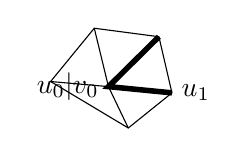
\begin{tikzpicture}[scale=.72]
\coordinate (a) at (0,.7);\coordinate (b) at (.77,1.64);\coordinate (c) at (1.91,1.49);\coordinate (d) at (2.14,.5);\coordinate (e) at (1.37,-.12);\coordinate (o) at (1.02,.61);
\draw (a)--(b)--(c)--(d)--(e)--cycle;
\draw (a)--(o)--(e) (b)--(o);\draw[line width=2pt] (c)--(o)--(d);
\node[left] at (o){$\unsure{u_0|v_0}$};\node[right] at (d){$u_1$};
\end{tikzpicture}}

\uline{Prop} Soient $u,v\in S_\alpha$, avec $v\ne u,u'$ Alors

\[
\begin{aligned}
\operatorname{Tr}v\,u^i(v)&=\alpha &&\text{si }i\deleted{\unsure{\ne}}\equiv1\text{ ou }-1\quad(5)\\
\operatorname{Tr}v\,u^i(v)&=\alpha' &&\text{si }\unsure{i'|i}\equiv2\text{ ou }-2\quad(5)\\
(&=1&&\text{si }i\equiv0\quad(5))
\end{aligned}
\]

\[
\begin{aligned}
\operatorname{Tr}uv_0&=1+\alpha(\lambda+\lambda^{-1})=1+\alpha=\alpha' &u^5&=\alpha\\
\unsure{T|\operatorname{Tr}}u\,v'_0&=\alpha
\end{aligned}
\]

\[
uv=\begin{pmatrix}1&0\\\alpha'&\alpha'\end{pmatrix}\qquad
u^{-1}v=\begin{pmatrix}0&1\\1&\alpha^{\unsure{2|{}|'}}\end{pmatrix}
\]

\[
\begin{aligned}
u_{\unsure{*|{}}}&=\begin{pmatrix}0&1\\\alpha&1\end{pmatrix}
&u^{-1}&=\begin{pmatrix}\alpha'&\alpha'\\1&0\end{pmatrix}\\
v_0&=\begin{pmatrix}1&\alpha\\1&0\end{pmatrix}\\
v_1&=uvu^{-1}=\begin{pmatrix}\alpha'&\alpha'\\1&\alpha^{\unsure{'|2|{}}}\end{pmatrix}\\
v_{-1}&=u^{-1}vu=\begin{pmatrix}\alpha&1\\\alpha^{\unsure{''|'}}&\alpha'\end{pmatrix}
\end{aligned}
\]

\figure{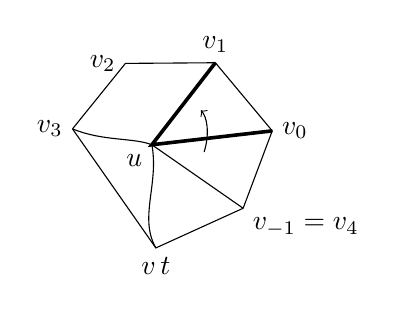
\begin{tikzpicture}[scale=.84]
\coordinate (a) at (-1.22,.1);\coordinate (b) at (-.42,1.09);\coordinate (c) at (.94,1.1);\coordinate (d) at (1.8,.07);\coordinate (e) at (1.36,-1.1);\coordinate (f) at (.04,-1.7);\coordinate (o) at (-.02,-.14);
\draw (a)--(b)--(c)--(d)--(e)--(f)--(a);
\draw (a)..controls(-.76,-.09)and(-.3,-.03)..(o)--(e) (f)..controls(-.22,-1.24)and(.09,-.74)..(o);
\draw[line width=1.3pt] (c)--(o)--(d);\draw[->] (.77,-.25) ..controls(.86,.04)and(.81,.29)..(.72,.38);
\node[left] at(a){$v_3$};\node[left] at(b){$\unsure{v_2}$};\node[above] at(c){$v_1$};\node[right] at(d){$v_0$};
\node[below right] at(e){$v_{-1}=v_4$};\node[below] at(f){$\deleted{\unsure{v}}\,t$};\node[below left] at(o){$u$};
\end{tikzpicture}}

\[
\begin{aligned}u^5&=\alpha\\(\alpha u)^5&=\alpha^6=1\\\det(\alpha u)&=\alpha^3=1\\&\deleted{\det}\end{aligned}
\]

val. propres de $u$ sont $\alpha,\alpha'$ \deleted{$\alpha u$}

\[
\begin{aligned}
\frac{12.11}{2}&=66=6+30+30\\
\frac{12.11.10}{6}&=\unsure{220|320}\\
&20+20+60+60\\
&\quad+6.10\\
&1+\alpha=\alpha'
\end{aligned}
\]

\[
\begin{aligned}
&\operatorname{Tr}\deleted{\unsure{v}}v\,uvu^{-1}=\alpha\\
&\deleted{\unsure{u=\lambda\eta}}\quad u'\quad\deleted{\unsure{u\alpha}}
\end{aligned}
\]

\figure{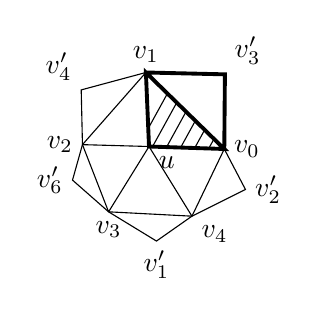
\begin{tikzpicture}[scale=.79]
\coordinate (u) at (0,0);\coordinate (a) at (1.21,-.04);\coordinate (b) at (-.05,1.19);\coordinate (c) at (-1.07,.03);\coordinate (d) at (-.65,-1.05);\coordinate (e) at (.69,-1.12);
\coordinate (aa) at (-1.23,-.54);\coordinate (bb) at (.12,-1.52);\coordinate (cc) at (1.55,-.69);\coordinate (dd) at (1.22,1.16);\coordinate (ee) at (-1.09,.91);
\draw (a)--(b)--(c)--(d)--(e)--cycle (u)--(c) (u)--(d) (u)--(e);
\draw (c)--(aa)--(d) (d)--(bb)--(e) (e)--(cc)--(a) (c)--(ee)--(b);
\draw[line width=1.4pt] (u)--(b)--(a)--cycle (b)--(dd)--(a);
\begin{scope}\clip (u)--(b)--(a)--cycle;\foreach \x in {-.2,.03,.26,.49,.72,.95}{\draw[thin] (\x,-.05)--++(.55,1);}\end{scope}
\node[below right] at(u){$u$};\node[right] at(a){$v_0$};\node[above] at(b){$v_1$};\node[left] at(c){$v_2$};\node[below] at(d){$v_3$};\node[below right] at(e){$v_4$};
\node[left] at(aa){$v'_{6}$};\node[below] at(bb){$v'_1$};\node[right] at(cc){$v'_2$};\node[above right] at(dd){$v'_3$};\node[above left] at(ee){$v'_4$};
\end{tikzpicture}}

$(u,v,w)$ forment un triangle,

\[
\det(u+v+w)=\underbrace{\det u+\det v+\det w}_{3\alpha=\alpha}
+\underbrace{\varphi(u,v)+\varphi(v,w)+\varphi(w,u)}_{\deleted{\unsure{\alpha'}}\quad3\alpha'=\alpha'}=1
\]

% archive sheet number: 15
